\documentclass[12pt, addpoints]{exam/exam}

\usepackage{hyperref}
%\usepackage{mdframed}
\usepackage{graphicx, caption}	
%\usepackage{array, multicol, tabu}
\usepackage{amsmath, amsthm, amssymb}
\usepackage{comment}
\usepackage{enumitem}
\usepackage{url}
\usepackage{textcomp}
\newcommand{\vect}[1]{\mathbf{#1}}
\newcommand{\R}{\mathbb R}
\newcommand{\vstr}{\vspace{\stretch{1}}}
\everymath{\displaystyle}
\setlength{\parindent}{0pt}

\theoremstyle{plain}
\newtheorem{thm}{Theorem}
\newtheorem*{thm*}{Theorem}

%\printanswers
\pointformat{\bf(\thepoints)}
\pointpoints{pt}{pts}
\bonuspointformat{\bf(\thepoints)}
\bonuspointpoints{pt}{pts}

\coverfirstpageheader{\bf MATH 2574 (Calculus III) \\
		Spring 2017 \\
		}
		{}
		{{Name:} \underline{\hspace{40ex}} \\
		\vspace{0.5pc}
		Wed 15 Mar 2017}
\coverextraheadheight[2pc]{0in}
\coverfirstpagefooter{}{}{\Large Good luck!}
\coverrunningheader{}
	{Exam 2: Multivariate derivatives and multiple integrals}
	{}
\coverrunningheadrule	
\coverrunningfootrule
\coverrunningfooter{Wheeler}{Cal III Spring 2017}{p. \thepage\ (of \numpages)}

\firstpageheader{}
	{Exam 2: Multivariate derivatives and multiple integrals}
	{}
\firstpageheadrule
\firstpagefootrule
\firstpagefooter{Wheeler}{Cal III Spring 2017}{p. \thepage\ (of \numpages)}

\runningheadrule
\runningheader{}
	{Exam 2: Multivariate derivatives and multiple integrals}
	{}
\runningfootrule
\runningfooter{Wheeler}{Cal III Spring 2017}{p. \thepage\ (of \numpages)}

\title{\vspace{-8pc}
\vfill{\Huge
	\bf Exam 2: Multivariate Derivatives \\ and Multiple Integrals \\ (\S 12.3-12.9, 10.1-10.3, 13.1-13.5)} 
	}
%\author{}
\date{}

% % % % % % % % % % % % % % % % % % % %
\begin{document}

\begin{coverpages}
\maketitle
\thispagestyle{headandfoot}
\vspace{-4pc}
{\bf Exam Instructions:} You have 50 minutes to complete this exam.  Justification is required for all problems.  %Notation matters!  You will also be penalized for missing units and rounding errors.  
No electronic devices (phones, iDevices, computers, etc) except for a \textbf{basic scientific calculator}.  On story problems, round to one decimal place. If you finish early then you may leave, UNLESS there are less than 5 minutes of class left.  To prevent disruption, if you finish with less than 5 minutes of class remaining then please stay seated and quiet.

\begin{flushright}
In addition, please provide the following data:

\vspace{0.3in}
Drill Instructor: \underline{\hspace{40ex}}

\vspace{0.3in}
Drill Time: \underline{\hspace{40ex}}
\end{flushright}

\vfill
\textbf{Your signature below indicates that you have read this page and agree to follow the Academic Honesty Policies of the University of Arkansas.}  

\vspace{0.3in}
Signature: {\bf (1 pt)} \underline{\hspace{73ex}}

% % % % % % % % % %
\newpage

\begin{center}
\vspace*{\fill}
%\gradetable
\vspace*{\fill}
\end{center}
\end{coverpages}

% % % % % % % % % % % % % % % % % % % %
\begin{questions}
\thispagestyle{headandfoot}

% % % % %
\question %{\bf \S10.2 \#61}
Determine whether the following statements are true or false.  You must justify your answer.
\begin{parts}
	% % %
	\part[4] The graphs of 
	%$r=2$ 
	$r=3$
	and 
	%$\theta=\frac{\pi}{4}$ 
	$\theta=\frac{\pi}{3}$
	intersect exactly once.
	\vspace{14pc}
	
	% % %
	\part[4] The graphs of 
	%$r=2\sec{\theta}$ 
	$r=4\sec{\theta}$
	and 
	%$r=3\csc{\theta}$ 
	$r=\csc{\theta}$
	are lines.
	\vspace{15pc}
	
	% % %
	\part[4] The point $\left(3,\frac{\pi}{2}\right)$ lies on the graph of $r=3\cos{2\theta}$.
	\vspace{15pc}
\end{parts}

\newpage
% % % % %
\question[12] %{\bf \S12.8 \#48}
Find the absolute maximum and minimum values of the function 
\[
f(x,y)=x^2+y^2-2x-2y
\]
on the closed region $R$, bounded by the triangle with vertices $(0,0),\,(2,0),\,(0,2)$.

\newpage
% % % % %
\question[10] %{\bf \S10.3 \#34}
Find the area of the region inside the rose 
%$r=4\cos{2\theta}$ 
$r=2\sin{2\theta}$
and outside the circle 
%$r=2$.
$r=1$.  
\textit{(In case you need it, the half-angle formula is $\cos^2{x}=\frac{1+\cos{2x}}{2}$.)}  

\newpage
% % % % %
\question[8] %{\bf \S12.9 \#50}
The following figure shows the level curves for various $z=z_0$ of the function $f$, along with the constraint curve $g(x,y)=0$.  Estimate the maximum and minimum values of $f$ subject to the constraint.  At each point where an extreme value occurs, indicate the direction of $\nabla f$ and the direction of $\nabla g$.

\begin{center}
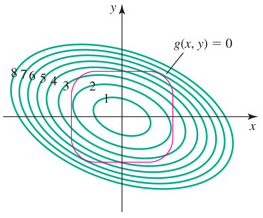
\includegraphics[scale=1.1]{12-9Exam2}
\end{center}
\vstr

% % % % % 
\question[6] %{\bf \S12.6 \#20}
Compute the directional derivative of 
\[
g(x,y)=\sin{(\pi(2x-y))}
\]
at the point $P=(-1,-1)$ in the direction of 
$\vect u=\langle \frac{5}{13},-\frac{12}{13}\rangle$.  
%$\vect u=\langle \frac{12}{13},-\frac{5}{13}\rangle$.
\vspace{22pc}

\newpage
% % % % % 
\question Evaluate (or show non-existence of) the following limits:
\begin{parts}
% % %
	\part[5] %{\bf \S12.3 \#64} 
	$\lim_{(x,y)\to(0,0)}\frac{xy}{|xy|}$
	%$\lim_{(u,v)\to(0,0)}\frac{|uv|}{uv}$
	\vspace{12pc}
	
	% % %
	\part[5] %{\bf \S12.3 \#54}	
	$\lim_{(x,y,z)\to(1,\ln 2,3)}(1+y)\ln{e^{xz}}$
	%$\lim_{(x,y,z)\to(\ln 2,3,1)}(1+x)\ln{e^{yz}}$
	\vspace{12pc}
\end{parts}

% % % % %
\question[6] %{\bf \S12.5 \#62}
The density of a thin circular plate of radius 2 is given by 
%$\rho(x,y)=4+xy$.  
$\rho(x,y)=3+xy$.
The edge of the plate is described by the parametric equations 
$x=2\cos t$, $y=2\sin t$, 
%$x=\cos t$, $y=\sin t$,
for $0\leq t\leq 2\pi$.	Find the rate of change of the density with respect to $t$ on the edge of the plate.



\newpage
% % % % %
\question[10] %{\bf \S13.5 \#70}
Set up, but \textbf{do not evaluate}, the integral for the volume of material remaining in a hemisphere of 
radius 2 
%radius 4
after a cylindrical hole of 
radius 1 
%radius 2
is drilled through the center of the hemisphere perpendicular to its base.
\vspace{1pc}

\textbf{ExTrA cReDiT (5 pts)} Evaluate the integral you set up.
 
\end{questions}

\end{document}